\section{Symbiosis}
Symbiosis brings Mitosis-Core and Mitosis-Stream all together and demonstrates with a very basic application how one would use it.
The sample application shall allow one user to broadcast a stream that is recorded with the camera of the device and $\ n $ other users shall be able to see the stream in real time.

\begin{figure}
\centering
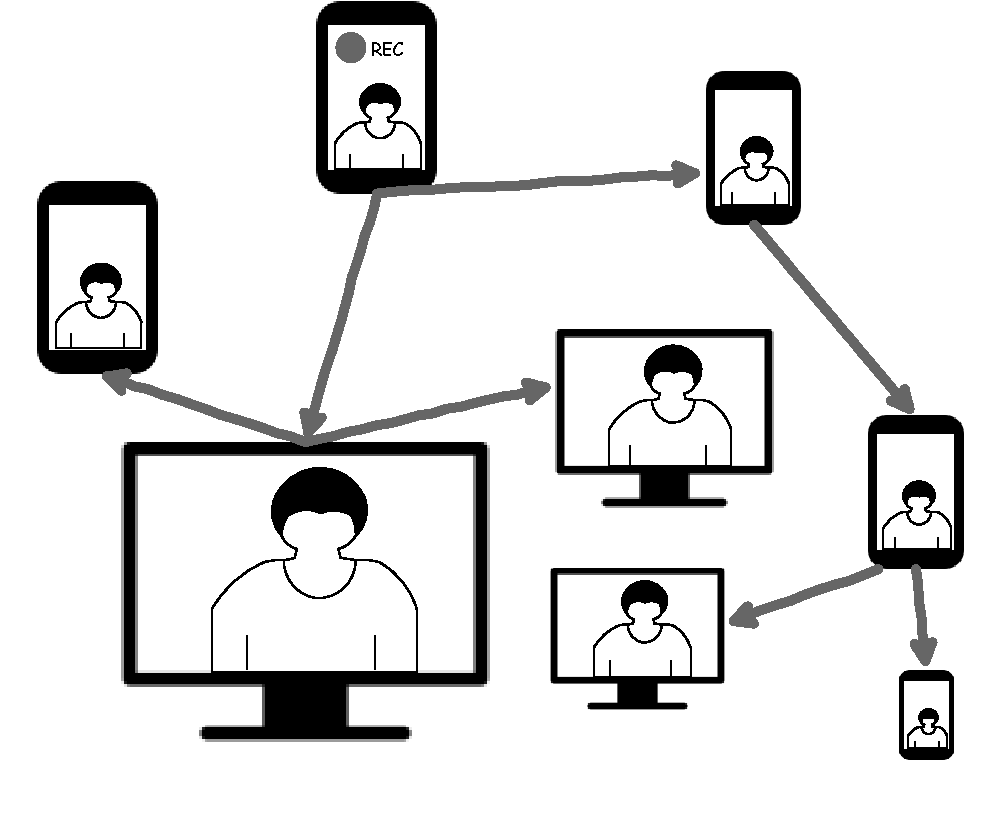
\includegraphics[width=0.75\textwidth]{graphics/implementation/symbiosis.pdf}
\caption{Symbiosis}
\label{fig:symbiosis-implementation}
\end{figure}

The \gls{ui} of the application has an \gls{html} VideoElement and a record button. When the user presses the record button the device starts the camera and waits for the stream. When the camera is ready the stream is set on the StreamManager (\vref{lst:symbiosis-start-stream}).

\begin{Listing}
\begin{lstlisting}
navigator.mediaDevices.getUserMedia({
    video: true,
    audio: false
  }).then(
    (stream) => {
      mitosis.getStreamManager().setLocalStream(stream);
    });
\end{lstlisting}
\caption{Access user camera and set stream}
\label{lst:symbiosis-start-stream}
\end{Listing}

The application is also listening for incoming streams. Users that have already started the application will get notify about the stream and it will start playing. When a user joins later and another user has already started broadcasting she will get the stream as well.
To allow the application to display the stream it has to observe the ChannelManger. When a channel is added it has to observe the channel for a stream. When the stream is available it can set the stream on the HTML VideoElement and start playing (\vref{lst:symbiosis-observe-stream}).

\begin{Listing}
\begin{lstlisting}
mitosis
  .getStreamManager()
  .observeChannelChurn()
  .subscribe(
    channelEv => channelEv.value
      .observeStreamChurn()
      .subscribe(
        streamEv => videoEl.srcObject = streamEv.stream;
      )
  );
\end{lstlisting}
\caption{Observe ChannelManager for incoming streams}
\label{lst:symbiosis-observe-stream}
\end{Listing}

The source-code for the whole application can be seen in \vref{sec:symbiosis-soruce-code}.